\documentclass[aspectratio=169,11pt,hyperref={colorlinks=true}]{beamer}
\usepackage[utf8]{inputenc}
\usepackage[T1]{fontenc}
\usepackage{fontspec}
\usepackage[absolute,overlay]{textpos}
\usepackage{listingsutf8}
\usepackage{listings-golang}
\usepackage{tikz}
\usepackage{color}


\title{Cloud Native CI/CD with Knative and Tekton Pipelines}
\date[devoxxfr]{April 18th 2019}
\author[Andrea]{
  Andrea Frittoli \\
  Developer Advocate \\
  andrea.frittoli@uk.ibm.com \\
  @blackchip76
}
\institute[devoxxfr]{
  Devoxx France, 8ème édition
}

\usetheme{ibmcloud}

% Code style
\setlststyle

\lstdefinelanguage{koyaml}{
  keywords={github, com, afrittoli, examples, ms, go, helloworld},
  sensitive=false,
  comment=[l]{\#},
  morestring=[b]',
  morestring=[b]"
}

% Automatic section frame
\AtBeginSection{\frame{\sectionpage}}

\begin{document}

\begin{frame}[noframenumbering]
\titlepage{}
\end{frame}

% The main points of the talk are:
% - give an introduction to Tekton Pipelines
% - get in some more details with an example
% - talk about Kaniko and source to image with tricky bits
% - reusing tasks, dev vs CI vs CD
% - point of integration with serving and eventing
% - can I use Tekton? Where? security concerns

% The slide/section order does not match the narrative yet

% Devoxx Talk structure

%% A bit of history
% Knative slide
% Community
%% An intro to knative serving
% A slide on serving, graph + scale up, down, traffic routes
% The OpenStack Health slide
%% Demo
% kubectl get all -n dev, kubectl get pods -n dev --watch
%% An intro to knative eventing
% A slide or two on eventing, existing framework, v5 slide?
%% Demo, submit a patch to github, watch the event log
%% Knative Build and Pipelines
% A slide on build, code sample, source to service type of experience
% Slide with complex pipeline
% knative build pipelines slide
% latest news slide
%% Tekton Pipeline
% Cloud Native Pipelines diagram
% Source to Image / Using Kaniko
% Diagram of the CD pipeline (I/O/DAG slide reworked)
% - title to CD pipeline
% CD Pipeline as Code (remove security?)
%% Under the Hood
% Custom resources
% Pods, Entrypoints and Volumes
%% Knative Serving and Tekton
% Pipelines and Knative Build slide
% CI With Tekton Pipelines reworked
% - "CI" application is a triggers
% - manual trigger for the development workflow
% - diagram from I/O/DAG
% KService for Health Frontend
%% Demo
% Push a change, run run_from_git.sh
%% Knative Eventing and Tekton
% Triggering and Knative Eventing / Asynchronous Pipelines
%% Conclusions

\section{A Bit of History}

\begin{lblackrwhiteframe}
  \frametitle{Knative}
  \large
  \begin{beamercolorbox}[wd=0.3\paperwidth]{text}
    \begin{itemize}
      \item Beginning of 2018...
      \item Knative:
      \begin{itemize}
        \item Build
        \item Eventing
        \item Serving
      \end{itemize}
    \end{itemize}
    \begin{itemize}
      \item OpenSource
      \item Contributors:
      \begin{itemize}
        \item Google
        \item Pivotal
        \item IBM
        \item RedHat
        \item Cloudbees
        \item ...and others
      \end{itemize}
    \end{itemize}
  \end{beamercolorbox}%
  \begin{textblock*}{0.5\paperwidth}(0.5\paperwidth,0.2\paperheight)
    \centering
    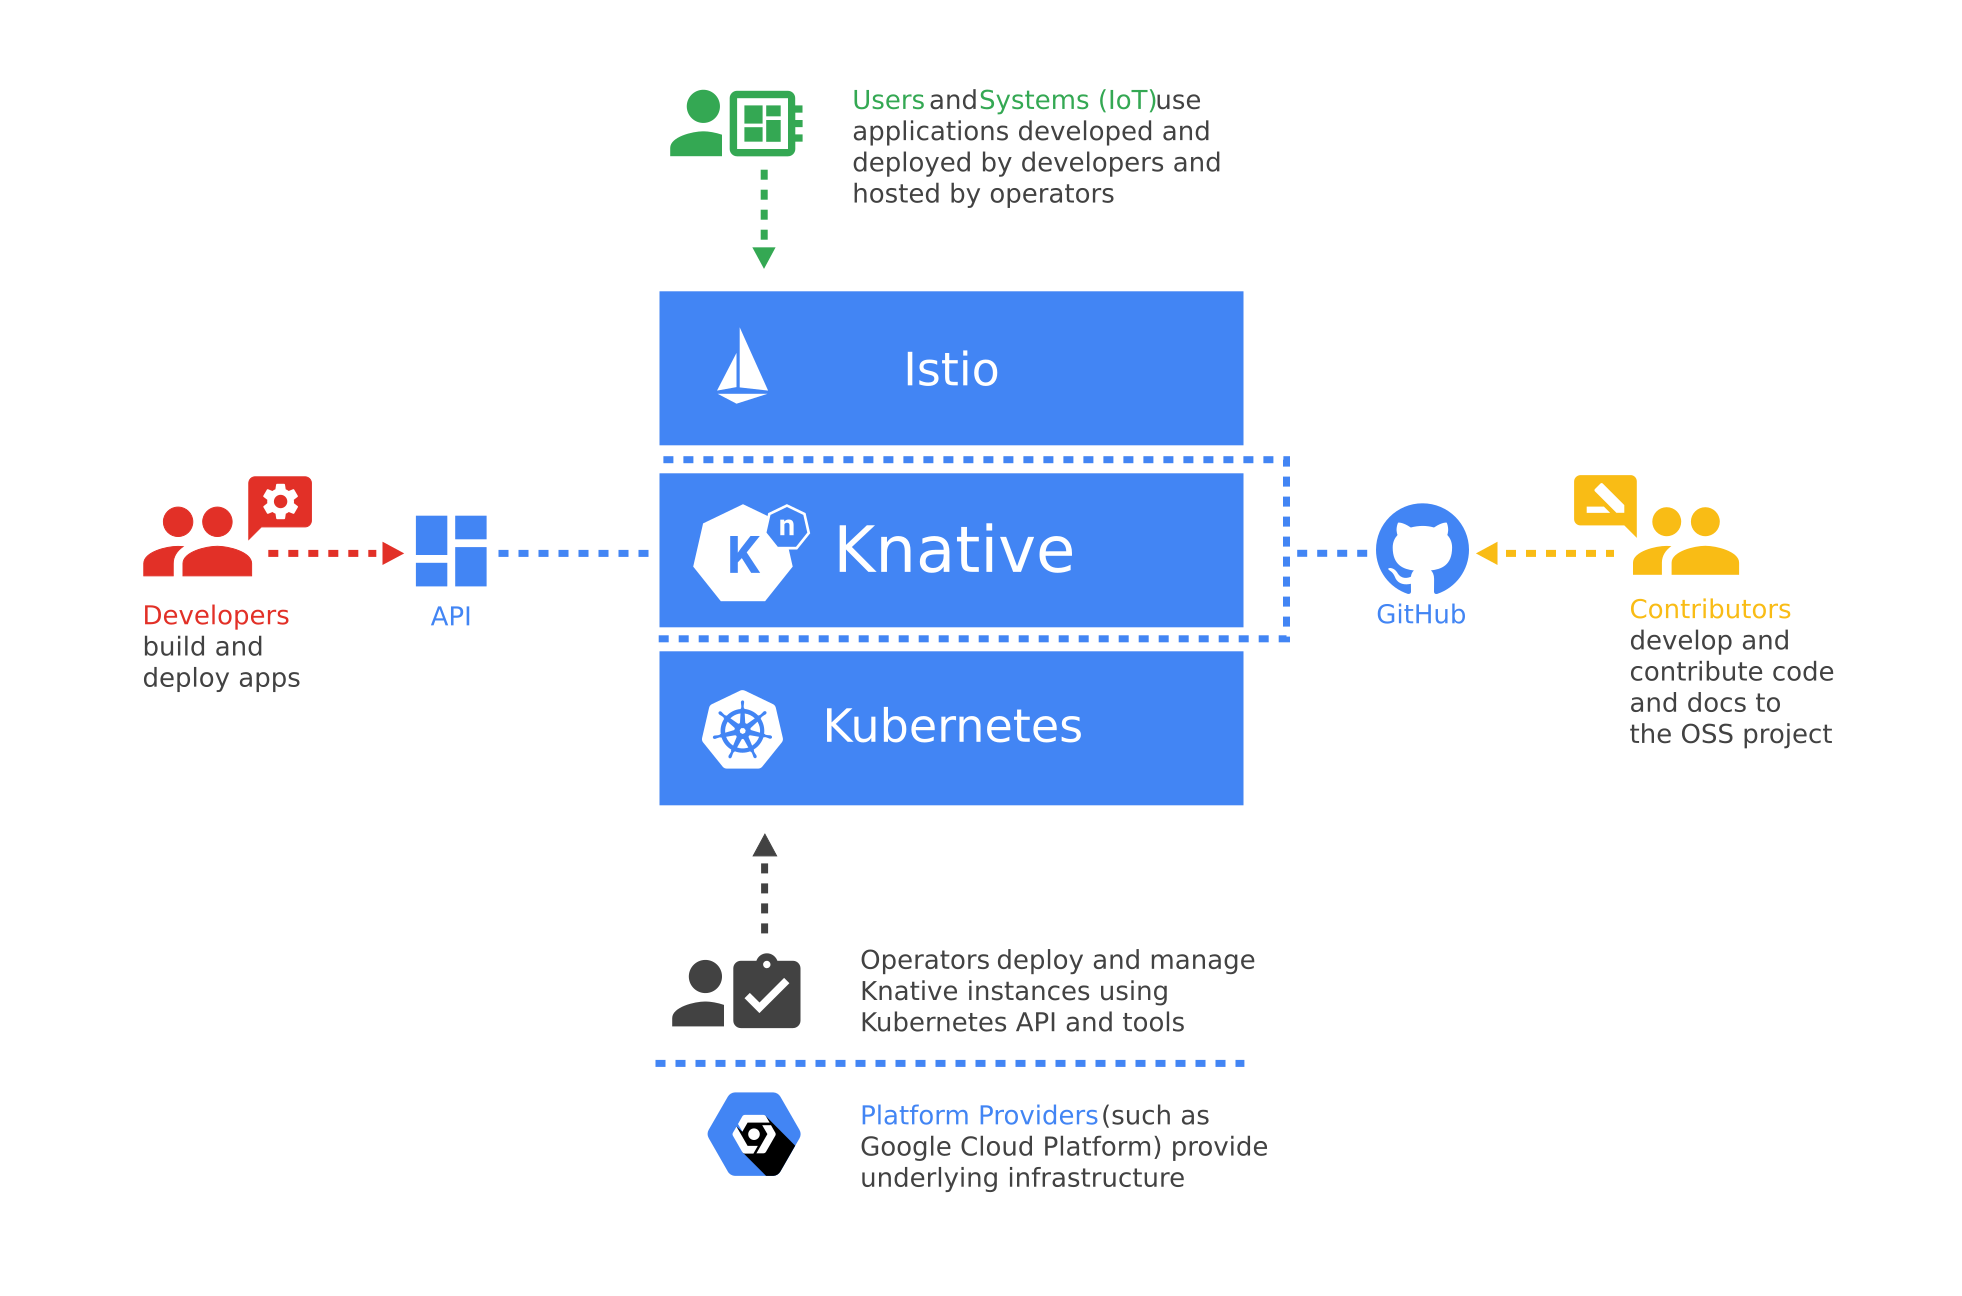
\includegraphics[width=0.45\paperwidth]{img/knative-audience.png}
  \end{textblock*}
\end{grayframe}

\begin{grayframe}
  \frametitle{Community}
  \begin{itemize}
    \item Steering Commitee (SC)
    \item Technical Oversight Commitee (TOC)
    \item Dedicated Working Groups (WG)
    \item Various Contribution profiles
    \item Design, issues: on GitHub
    \item Communication:
    \begin{itemize}
      \item WG periodic meetings, recorded
      \item Asynch: Knative Users / Developers ML
      \item Sync: slack.knative.dev
    \end{itemize}
  \end{itemize}
\end{grayframe}

\section{Knative Serving}

\begin{lblackrwhiteframe}
  \frametitle{Knative Serving}
  \begin{beamercolorbox}[wd=0.4\paperwidth]{text}
    \begin{itemize}
      \item Scale to Zero
      \item Scale up based on metrics
      \item Multiple revisions
    \end{itemize}
  \end{beamercolorbox}%
  \begin{textblock*}{0.5\paperwidth}(0.5\paperwidth,0.2\paperheight)
    \centering
    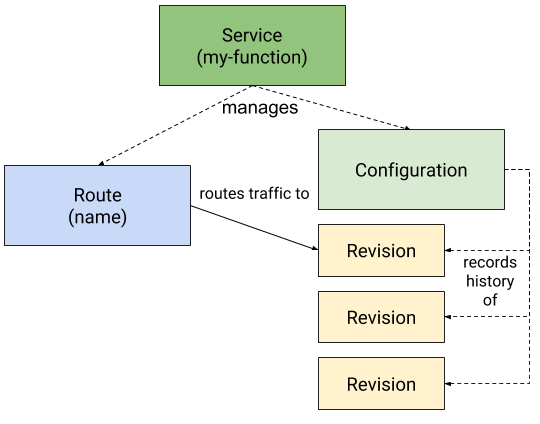
\includegraphics[width=0.45\paperwidth]{img/knative-serving.png}
  \end{textblock*}
\end{tblackbgrayframe}

\begin{grayframe}
  \frametitle{The Health Application}
  % Talk about the architecture and git repos
  \begin{textblock*}{\paperwidth}(0cm,0cm)
    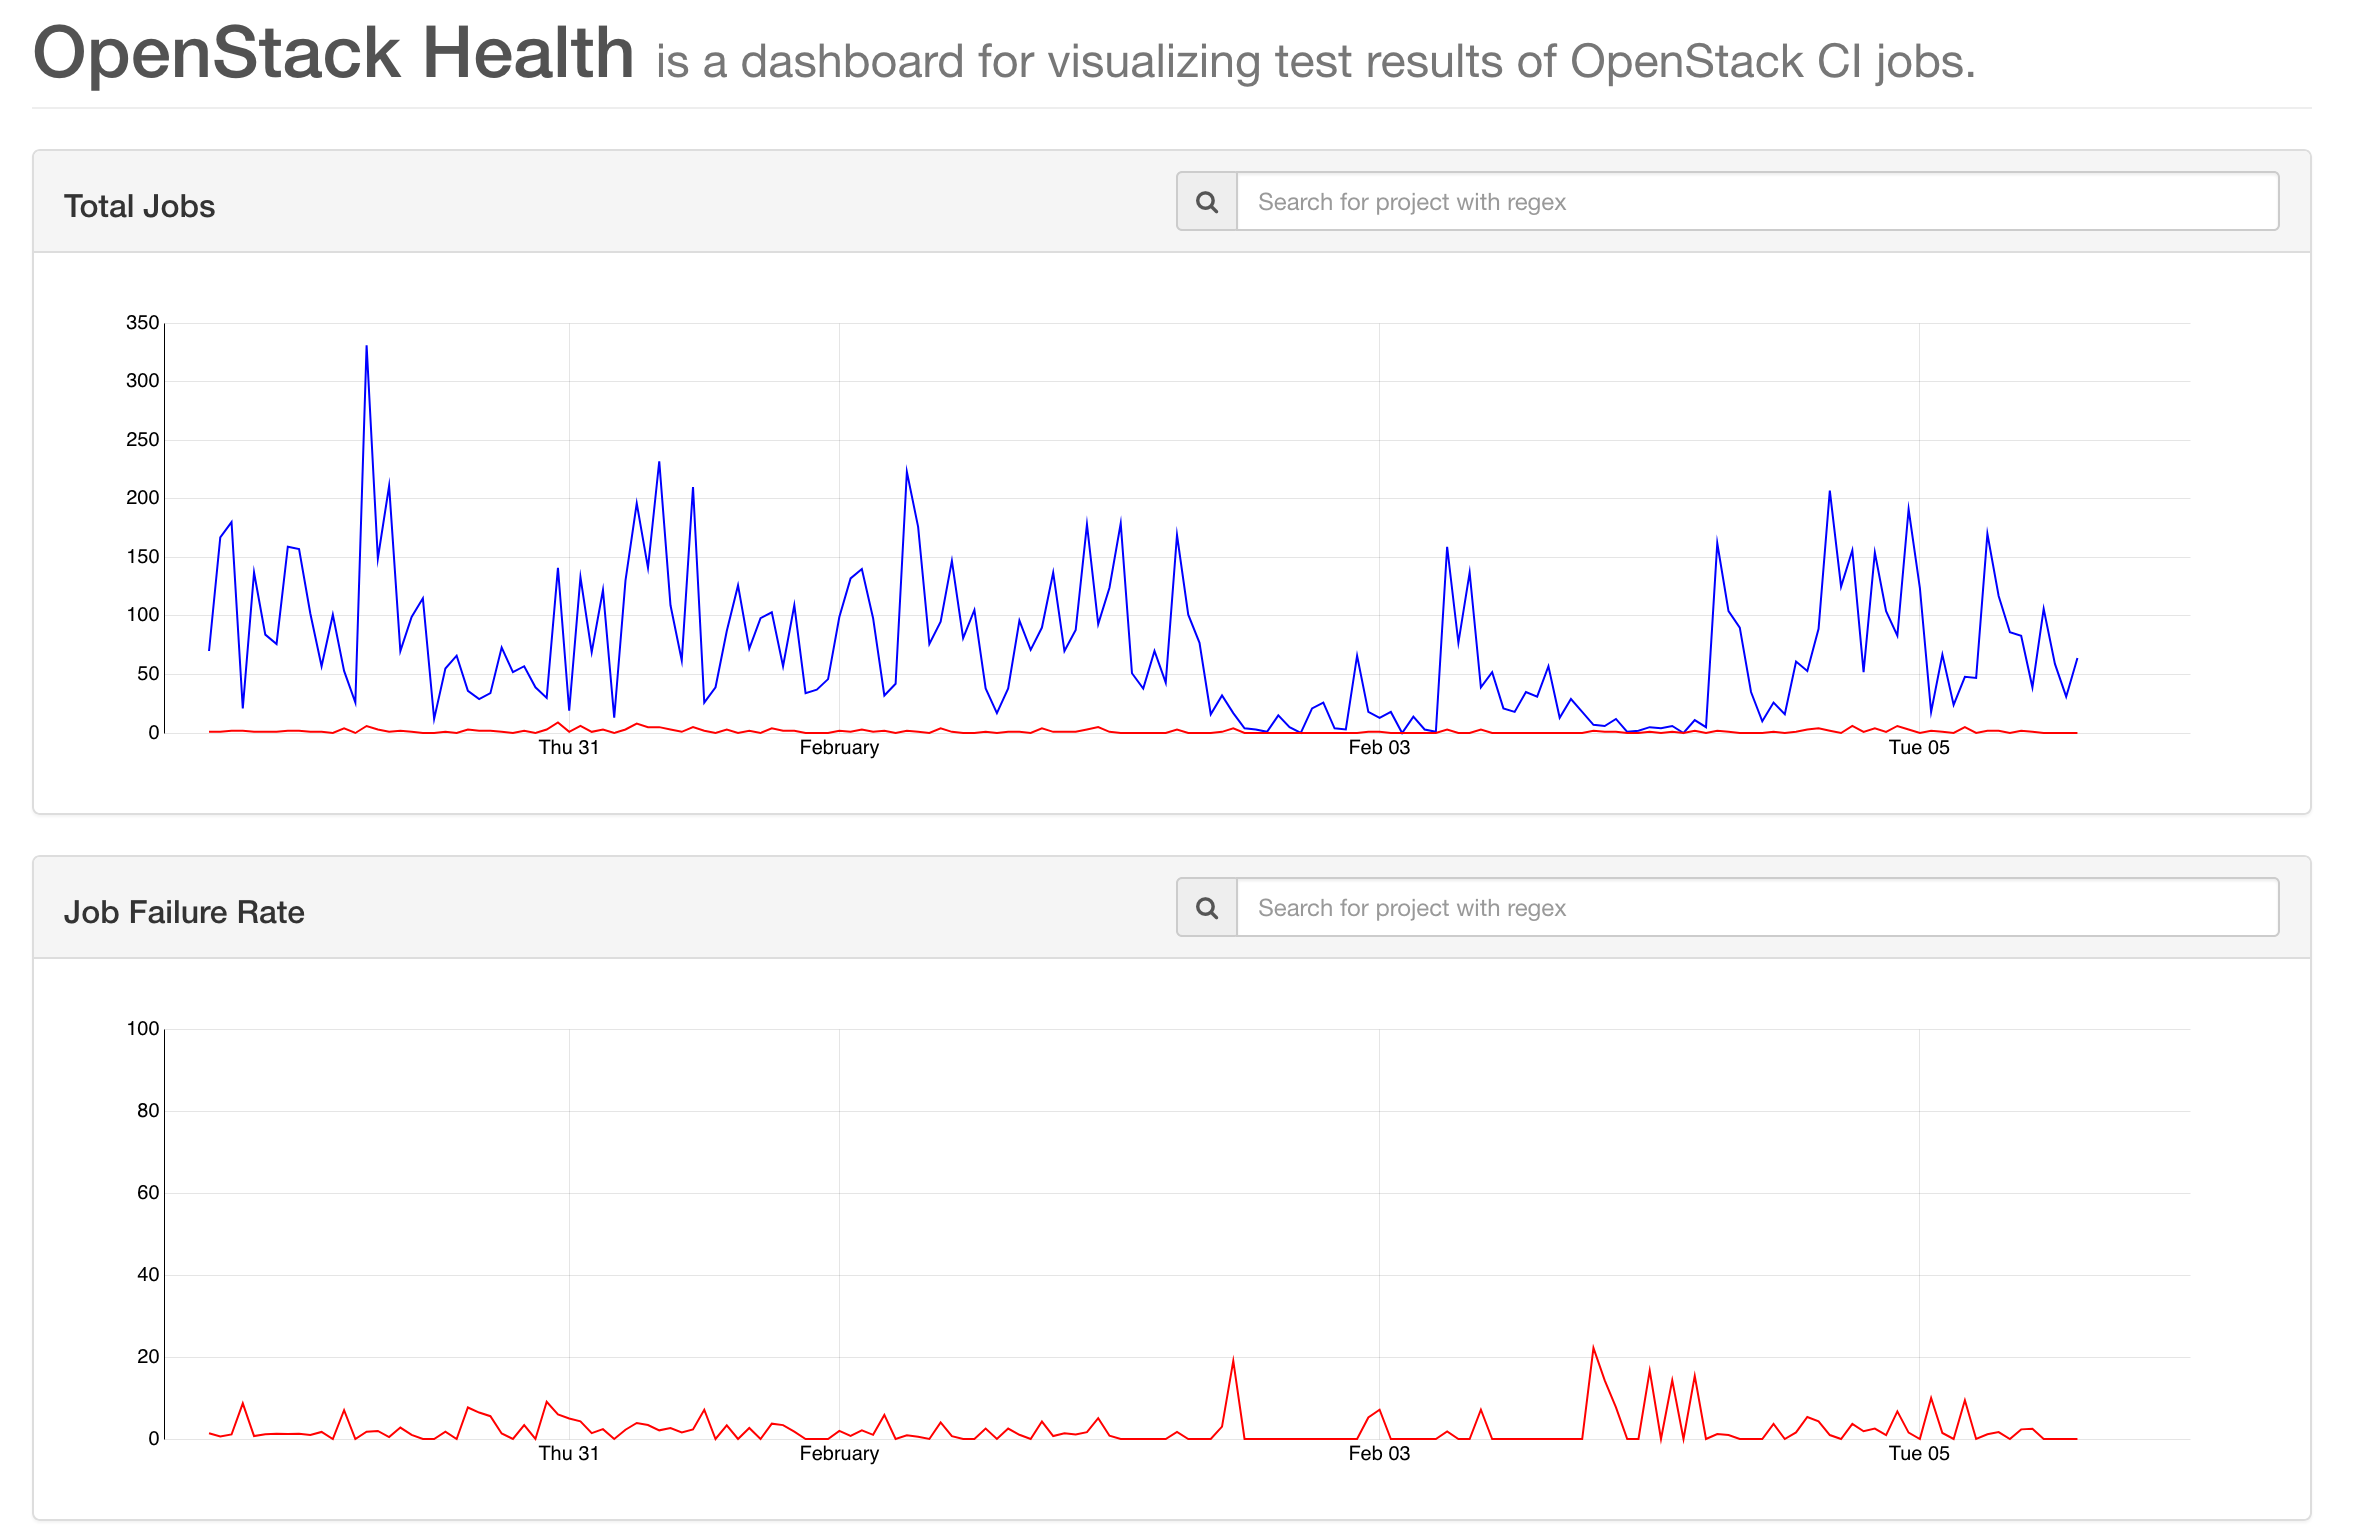
\includegraphics[width=\paperwidth, height=\paperheight]{img/openstack-health.png}
  \end{textblock*}
  \begin{textblock*}{0.2\paperwidth}(0.83\paperwidth,0.83\paperheight)
    
\includegraphics[width=0.03\paperwidth]{img/cc.png}
    
\includegraphics[width=0.03\paperwidth]{img/zero.png}
  \end{textblock*}
\end{grayframe}

\section{Knative Serving Demo}
% kubectl get all -n dev
% kubectl get pods -n dev --watch
% curl [API end point]
% curl [FE endpoint]
% Show in browser
% ...later: show scale back down to zero

\section{Knative Eventing}

\begin{tblackbgrayframe}
  \frametitle{Knative Eventing}
  \begin{textblock*}{\paperwidth}(0.32cm,0.2\paperheight)
    \centering
    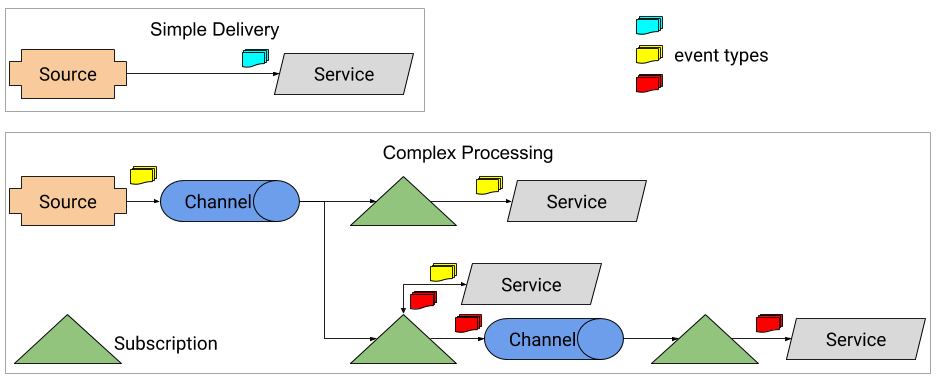
\includegraphics[width=0.9\paperwidth]{img/eventing-control-plane.png}
  \end{textblock*}
  % Talk about events as triggers for serverless services
  % Sources: git, k8s events
  % Channel: in memory, kafka, others
  % Subscriptions: service to a channel
  % v5: Brokers and Triggers
\end{tblackbgrayframe}

\section{Knative Eventing Demo}
% submit a patch to github, watch the event log

\section{Knative Build and Pipelines}

\begin{2columnsframe}
  {
  \begin{itemize}
    \item Source to image
    \item Build Templates
    \item How to make a new revision
  \end{itemize}
  }
  {
  \lstinputlisting[language=koyaml,firstline=1,lastline=25]{code/source-to-url-go.yaml}
  }
  \frametitle{Knative Build}
\end{2columnsframe}

\begin{tblackbgrayframe}
  \frametitle{Going further}
  \begin{textblock*}{0.75\paperwidth}(0.15\paperwidth,0.25\paperheight)
    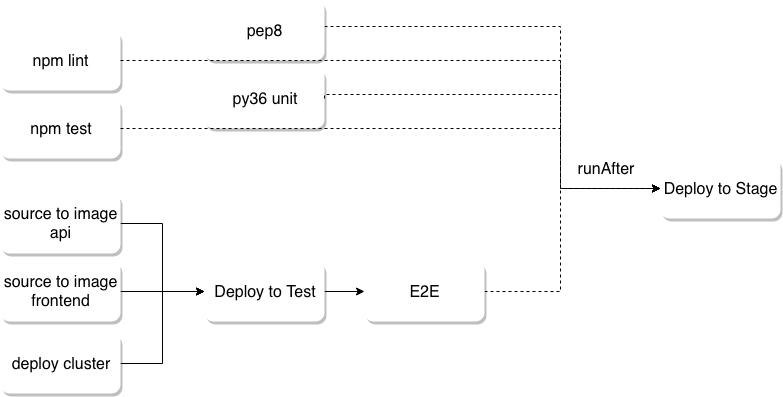
\includegraphics[width=0.75\paperwidth]{img/test-pipeline.png}
  \end{textblock*}
\end{tblackbgrayframe}

\begin{blackframe}
  \frametitle{\textasciitilde Sept 2018: Knative Pipelines}
  \begin{textblock*}{\paperwidth}(0cm,0.2\paperheight)
    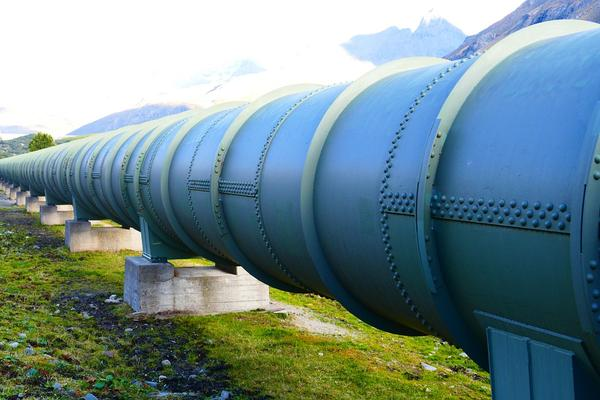
\includegraphics[width=\paperwidth]{img/pipeline_cc0.jpg}
    % https://mediad.publicbroadcasting.net/p/shared/npr/styles/placed_wide/nprshared/201804/605180710.jpg
  \end{textblock*}
  \begin{textblock*}{0.2\paperwidth}(0.83\paperwidth,0.93\paperheight)
    
\includegraphics[width=0.03\paperwidth]{img/cc.png}
    
\includegraphics[width=0.03\paperwidth]{img/zero.png}
  \end{textblock*}
\end{blackframe}

\begin{lblackrwhiteframe}
  \frametitle{Latest news!}
  \large
  \begin{beamercolorbox}[wd=0.3\paperwidth]{text}
    \begin{itemize}
      \item Tekton pipelines
      \item Focus on CI/CD
      \item @CD Foundation
      \item Deploy ``anywhere''
      \item ``Compatible'' with Knative
    \end{itemize}
  \end{beamercolorbox}%
  \begin{textblock*}{0.5\paperwidth}(0.5\paperwidth,0.25\paperheight)
    \centering
    
\includegraphics[width=0.35\paperwidth]{img/tekton-horizontal-color.png}
    
\includegraphics[width=0.20\paperwidth]{img/cdf-color.png}
  \end{textblock*}
\end{lblackrwhiteframe}

\section{Tekton Pipelines}

\begin{blackframe}
  \frametitle{Cloud Native Pipelines}
  % Cloud Native Pipelines, run on Kubernetes
  \begin{textblock*}{\paperwidth}(0.05\paperwidth,0.2\paperheight)
    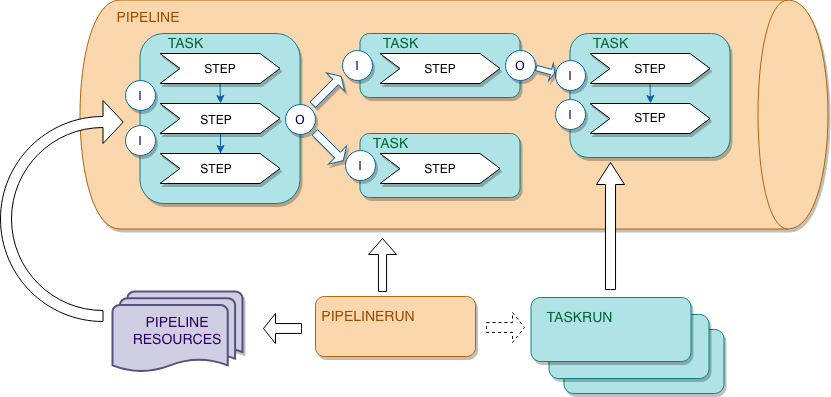
\includegraphics[width=0.85\paperwidth]{img/tekton.png}
  \end{textblock*}
  \begin{textblock*}{0.2\paperwidth}(0.9\paperwidth,0.83\paperheight)
    
\includegraphics[width=0.03\paperwidth]{img/cc.png}
    
\includegraphics[width=0.03\paperwidth]{img/zero.png}
  \end{textblock*}
\end{grayframe}

\begin{2columnsframe}
  {
    \begin{itemize}
      \item Steps are sequential
      \item Tasks are a Directed Acyclic Graph
      \item Order defined by:
      \begin{itemize}
        \item {\em from}: input / output
        \item {\em runAfter}: enforced ordering
      \end{itemize}
    \end{itemize}
  }
  % Graph of a CD pipeline
  {
  \begin{textblock*}{0.65\paperwidth}(0.30\paperwidth,0.30\paperheight)
    \centering
    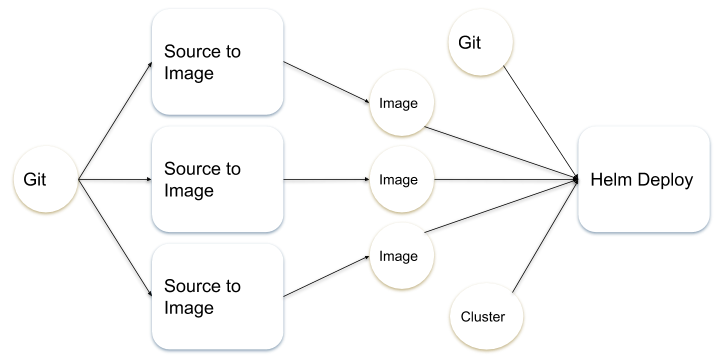
\includegraphics[width=0.65\paperwidth]{img/pipeline.png}
  \end{textblock*}
  }
  \frametitle{Task Inputs, Outputs \& DAG}
\end{2columnsframe}

\begin{2columnsframe}
  {
  {\tiny Source to Image (spec only): \\}
  \lstinputlisting[language=koyaml,firstline=6,lastline=31]{code/task-source-to-image.yaml}
  }
  {
  \lstinputlisting[language=koyaml,firstline=32,lastline=55]{code/task-source-to-image.yaml}
  {\tiny Cache Warmer (spec only): \\}
  \lstinputlisting[language=koyaml,firstline=21,lastline=35]{code/task-kaniko-cache.yaml}
  }
  \frametitle{Source to Image with Kaniko}
\end{2columnsframe}

\begin{lblackrwhiteframe}
  \frametitle{Using Kaniko}
  \large
  \begin{beamercolorbox}[wd=0.45\paperwidth]{text}
    \begin{itemize}
      \item Features:
      \begin{itemize}
        \item Build from Context and Dockerfile
        \item Unpriviledged
        \item Reproducible
        \item Remote caching of layers
        \item Base images caching (warmer)
      \end{itemize}
    \end{itemize}
    \vspace{3ex}
    \begin{itemize}
      \item Dockefile?
      \begin{itemize}
        \item Most common changes last
        \item Careful with COPY/ADD
        \item Remove what you don't need
      \end{itemize}
    \end{itemize}
  \end{beamercolorbox}%
  \begin{textblock*}{0.5\paperwidth}(0.5\paperwidth,0.30\paperheight)
    \centering
    
\includegraphics[width=0.35\paperwidth]{img/Kaniko-Logo.png}
  \end{textblock*}
\end{lblackrwhiteframe}

\begin{2columnsframe}
  {
  \begin{itemize}
    \item Pipeline and Tasks in git (YAML)
    \item Parameters for env/run specific
    \item Security?
  \end{itemize}
  \vspace{3ex}
  \lstinputlisting[language=koyaml]{code/resource-git.yaml}
  }
  {
  \lstinputlisting[language=koyaml]{code/resource-cluster.yaml}
  \vspace{1ex}
  \lstinputlisting[language=koyaml]{code/resource-image.yaml}
  }
  \frametitle{CD Pipeline as code}
\end{2columnsframe}

\section{Under the Hood}

\begin{grayframe}
  \frametitle{Custom Resources}
  CRDs: Task(Run), Pipeline(Run), PipelineResource \\
  \vspace{3ex}
  Services in the {\em tekton-pipelines} namespace:
  \begin{itemize}
    \item Webhook Service: resource validation
    \item Controller Service:
    \begin{itemize}
      \item Handles inputs and outputs
      \item Calculates the DAG
      \item Provisions pods and containers
    \end{itemize}
  \end{itemize}
  \vspace{3ex}
  Custom Resource Provisioning:
  \begin{itemize}
    \item Via YAML
    \item Via Go API
    \item Labels!
  \end{itemize}
\end{grayframe}

\begin{2columnsframe}
  {
  Steps (of a Task):
  \begin{itemize}
    \item Containers in one POD (single node)
    \item Any container image
    \item Entrypoint re-written
    \item Serial execution
    \item Resource allocation?
  \end{itemize}
  \vspace{3ex}
  TaskRun:
  \begin{itemize}
    \item Provisions a POD
    \item Deployes entrypoint tool
    \item Input/output containers
    \item User containers (steps)
  \end{itemize}
  }
  {
  Volumes:
  \begin{itemize}
    \item EmptyDir for workspace/home
    \item Tools (entrypoint)
    \item Secrets
    \item Any user ConfigMap / Volume
    \item (Optionally) Pipeline Share
  \end{itemize}
  \vspace{3ex}
  PipelineRun:
  \begin{itemize}
    \item Several PODs, different nodes
    \item Shared storage: PVC or GCS
  \end{itemize}
  }
  \frametitle{Pods, Entrypoints \& Volumes}
\end{2columnsframe}

% \begin{lblackrwhiteframe}
%   \frametitle{IBM Cloud}
%   \large
%   \begin{beamercolorbox}[wd=0.4\paperwidth]{text}
%     \begin{itemize}
%       \item Private Registry:
%       \begin{itemize}
%         \item Tekon Images (push/pull)
%         \item User Images (push/pull)
%       \end{itemize}
%       \item Service Accounts:
%       \begin{itemize}
%         \item {\em tekton-pipelines-controller}
%         \item Pipeline/Task service account
%       \end{itemize}
%     \end{itemize}
%     \vspace{3ex}
%     \begin{itemize}
%       \item Knative @ IBM Cloud
%       \begin{itemize}
%         \item Experimental Add-on
%         \item {\em ibmcloud ks cluster-addon-enable knative}
%       \end{itemize}
%     \end{itemize}
%   \end{beamercolorbox}%
%   \begin{textblock*}{0.5\paperwidth}(0.5\paperwidth,0.3\paperheight)
%     \centering
%     
\includegraphics[width=0.35\paperwidth]{img/IBM-Cloud.png}
%   \end{textblock*}
% \end{lblackrwhiteframe}

\section{Tekton and Knative Serving}

\begin{grayframe}
  \frametitle{Pipelines and Knative Build}
  % *Run can be used as build with serving via duck typing
  % Build probably won't be developed much further
  % ...but you never know
  % Do something more complex with pipelines
  \begin{textblock*}{0.5\paperwidth}(0.20\paperwidth,0.30\paperheight)
    \centering
    
\includegraphics[width=0.6\paperwidth]{img/knative+tekton.png}
  \end{textblock*}
\end{grayframe}

\begin{lblackrwhiteframe}
  \frametitle{CI with Tekton Pipelines}
  % It's not a CI engine...
  % ...but it works well with one
  % Dogfooding
  % What about secrets?
  % Existing integrations
  % - jenkinsX, prow
  % - gitlab? pivotal? to be checked
  % - higher level abstractions
  \large
  \begin{beamercolorbox}[wd=0.45\paperwidth]{text}
    You need a ``CI`` application: \\
    \begin{itemize}
      \item Prow, JenkinsX, Zuul...
      \item Pipelines triggered by a CI app
      \item ...or by a developer
    \end{itemize}
    \vspace{3ex}
    Tekton to CI for Tekton (AKA Dogfooding) \textbackslash o/ \\
    \vspace{3ex}
    What about security?
    \begin{itemize}
      \item Malicious users
      \item Running a pipeline from a PR
      \item Access to secrets
    \end{itemize}
  \end{beamercolorbox}%
  \begin{textblock*}{0.5\paperwidth}(0.5\paperwidth,0.15\paperheight)
    \centering
    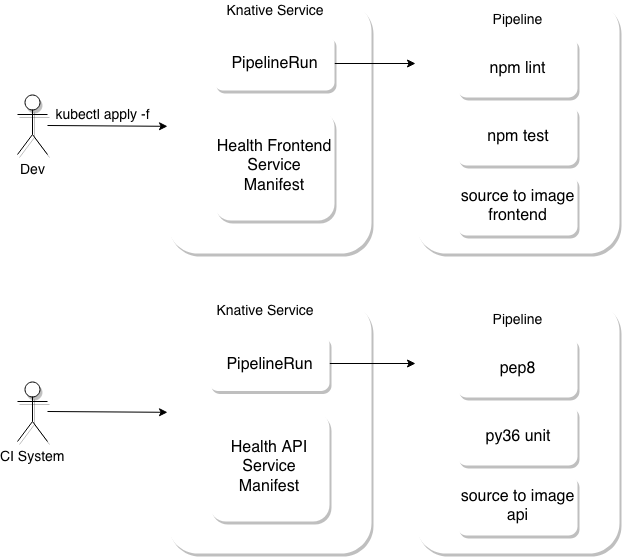
\includegraphics[width=0.45\paperwidth]{img/tekton_ci.png}
  \end{textblock*}
\end{lblackrwhiteframe}

\begin{2columnsframe}
  {
  \lstinputlisting[language=koyaml,firstline=1,lastline=27]{code/frontend.yaml}
  }
  {
  \lstinputlisting[language=koyaml,firstline=28,lastline=58]{code/frontend.yaml}
  }
  \frametitle{KService for Health Frontend}
\end{2columnsframe}

\section{Demo Tekton and Knative Serving}

\section{Asynchronous Pipelines}

\begin{2columnsframe}
  % Manual trigger
  % Using tasks and pipelines in Kservices
  % Native triggers: TBD
  % Async pipelines
  % GitHub events
  % -> push/pull request (CI)
  % -> comment (CI / CD)
  % -> release (CD)
  {
  \begin{itemize}
    \item Manual trigger for {\em PipelineRun}
    \item Native Eventing triggers TBD
    \item What about async pipelines?
    \begin{itemize}
      \item GitHub Source
      \item Container Source
      \item Pipeline Output as a Source
    \end{itemize}
  \end{itemize}
  }
  {
  \begin{textblock*}{0.6\paperwidth}(0.35\paperwidth,0.35\paperheight)
    \centering
    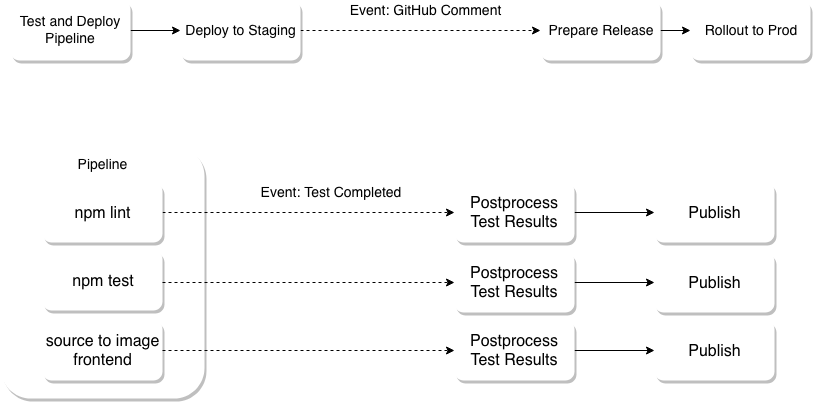
\includegraphics[width=0.6\paperwidth]{img/async_pipelines.png}
  \end{textblock*}
  }
  \frametitle{Triggering and Knative Eventing}
\end{2columnsframe}

% \begin{grayframe}
%   \frametitle{Tekton and Development}
%   \begin{itemize}
%     \item It depends.
%     \item What can go wrong?
%     \begin{itemize}
%       \item Building the container image
%       \item Provisioning and I/O of shared storage
%       \item Pipeline Output as a Source
%     \end{itemize}
%     \item What do I gain?
%     \begin{itemize}
%       \item Same building blocks used in CI/CD
%       \item Run in containers from the start
%       \item Parallel execution
%     \end{itemize}
%   \end{itemize}
%   % Maybe
%   % Local development with minikube
%   % Skaffold, ko, gulp
%   % Pros and cons
% \end{grayframe}

\section {Demo Tekton and Knative Eventing}
% # Make a code change
% git commit --amend
% git push origin devoxx_demo --force
% # See the event coming in
% kubectl logs $(kubectl get pods -l serving.knative.dev/configuration=github-message-dumper --no-headers -o custom-columns=":metadata.name") -c user-container
% # On the glue repo
% ko apply -f config
% kubectl get pods -l serving.knative.dev/github-tekton-glue
% # Make a change again
% git commit --amend
% git push origin devoxx_demo --force
% kubectl logs $(kubectl get pods -l serving.knative.dev/configuration=github-tekton-glue --no-headers -o custom-columns=":metadata.name") -c user-container
% # Run the watch command to see the pipeline running

\section{Conclusions}

\begin{grayframe}
  \frametitle{Conclusions}
  \begin{itemize}
    \item Tekton:
    \begin{itemize}
      \item Not only for knative
      \item Knative first class citizen
      \item Very early days
    \end{itemize}
    \item Tekton Roadmap:
    \begin{itemize}
      \item Conditional Execution
      \item Build Results and Logs
      \item Pluggable Tasks
      \item Triggering
      \item Community Library
    \end{itemize}
  \end{itemize}
\end{grayframe}

\begin{grayframe}
  \frametitle{References}
  \begin{itemize}
    \item This Talk: https://github.com/afrittoli/tekton\_pipelines\_knative\_intro
    \item Tekton Links:
    \begin{itemize}
      \item https://tekton.dev/, https://cd.foundation/
      \item https://github.com/tektoncd/pipeline
      \item https://github.com/tektoncd/pipeline
      \item https://github.com/tektoncd/pipeline/blob/master/api\_compatibility\_policy.md
      \item https://github.com/tektoncd/pipeline/blob/master/roadmap-2019.md
    \end{itemize}
    \item Knative Community: https://github.com/knative/docs/tree/master/community
    \item Kaniko: https://github.com/GoogleContainerTools/kaniko
    \item Source code and my blog:
    \begin{itemize}
      \item https://github.com/afrittoli/health-helm/tree/knative
      \item https://github.com/afrittoli/openstack-health/tree/knative-eventing
      \item https://github.com/afrittoli/github\_tekton\_glue
      \item https://andreafrittoli.me
    \end{itemize}
    \item IBM Cloud: https://cloud.ibm.com
  \end{itemize}
\end{grayframe}

\section{Q\&A}

\end{document}
